\documentclass[a4paper]{standalone}

% use this declaration to set specific page margins
%\usepackage[a4paper , lmargin = {2.7cm} , rmargin = {2.9cm} , tmargin = {2.7cm} , bmargin = {4.6cm} ]{geometry}
\usepackage[a4paper]{geometry}
\usepackage[ngerman, english]{babel}

\usepackage[utf8]{inputenc}
\usepackage[boxed]{algorithm2e}
\usepackage{amsmath}
\usepackage{amssymb}
\usepackage{authblk}
\usepackage{caption}
\usepackage{cleveref}
\usepackage [autostyle, english = american]{csquotes}
\usepackage{fontenc}
\usepackage{fontspec}
\usepackage{graphicx}
\usepackage[pagebackref=true]{hyperref}
\usepackage{multirow}
\usepackage[section]{placeins}
\usepackage{refstyle}
\usepackage{standalone}
\usepackage{subcaption}
\usepackage{tabularx}
\usepackage{url}
\usepackage{scrpage2}					% header and footer line


% header and footer line - no header & footer line on pages where a new chapter starts
\pagestyle{scrheadings}
\ohead{Mixing Text and Image Modalities in Artificial Neural Networks}
\ihead{Mario Tambos}
\ofoot[]{\thepage}
\ifoot{Master's Thesis, Mario Tambos, TU Berlin, Fachgebiet NI, 2018}

\MakeOuterQuote{"}

\newref{part}{name=part~,Name=Part~,names=parts~,Names=Parts~}
\newref{alg}{name=algorithm~,Name=Algorithm~,names=algorithms~,Names=Algorithms~}
\newref{sec}{name=section~,Name=Section~,names=sections~,Names=Sections~}
\newref{subsec}{name=subsection~,Name=Subsection~,names=subsections~,Names=Subsections~}

\newcommand{\vect}[1]{\mathbf{#1}}

\newcommand{\vecx}{\vect{x}}
\newcommand{\Dcal}{\mathcal{D}}
\newcommand{\Sbf}{\Sigma}
\newcommand{\Sbfs}{\Sigma^\star}
\newcommand{\Rbb}{\mathbb{R}}
\newcommand{\Nbb}{\mathbb{N}}

\makeatletter
\setlength{\@fptop}{0pt}
\makeatother

\makeatletter
\AtBeginDocument{%
    \expandafter\renewcommand\expandafter\subsection\expandafter{%
        \expandafter\@fb@secFB\subsection
    }%
}
\makeatother


\begin{document}
\section{Image retrieval}\label{sec:ImageRetrieval}

In this section we evaluate the performance of our model at an image retrieval task. Given a sequence of characters, a "query word" or "query sentence", we want to retrieve the associated images from a dataset of image-sentence pairs. 

Following the work of Karpathy, Joulin and Fei-Fei \cite{karpathy2014deep}, we decided to evaluate our model at this task using the Flickr8K\cite{young2014image} and Flickr30K datasets \cite{plummer2015flickr30k}. These datasets consist of images, each associated with 5 natural language sentences. The sentences are of variable length, and they describe what is occurring in the image. In each experiment in this section, 1000 images were extracted as a test set, and we trained our models on the rest. This resulted in 30783 training images, for the Flickr30K dataset, and 7092 training images, for the Flickr8K dataset.

For each dataset, we trained two different models on our experiments:
\begin{itemize}
    \item \texttt{MMSOM-Word}: we build new training and test sets by extracting all unique nouns in the five sentences corresponding to an image, and then creating image-noun pairs, rather than image-sentence pairs. The GloVe features used correspond to the embeddings of the the individual nouns. For the "flat hit @ k" measure, an image retrieved by the model was considered correct if the query word was present in any of the descriptions of the image.
    \item \texttt{MMSOM-Sentence}: we worked directly with image-sentence pairs. The GloVe features used correspond to the mean vector of the embeddings of the all individual words in a sentence, without any filtering of stop words. For the "flat hit @ k" measure, an image retrieved by the model was considered correct if the query sentence was among the description sentences of the image.
\end{itemize}

The resulting train and test sizes are shown in \figref{ImageRetrievalDatasetSizes} and \tabref{ImageRetrievalDatasetSizes}. \Figref{ImageRetrievalResults} shows the results we obtained on the test sets. \Tabref{ImageRetrievalResults} shows the same, for a detailed reference.

In all cases, the SOM models were trained using a grid of $100\times 100 = 10000$ units. Since we did not have a criterion clear enough for choosing the number of units, as is the case in \secref{ImageClassification}, we set a grid as big as our hardware setup allowed.

\begin{figure}[h]
    \centering
    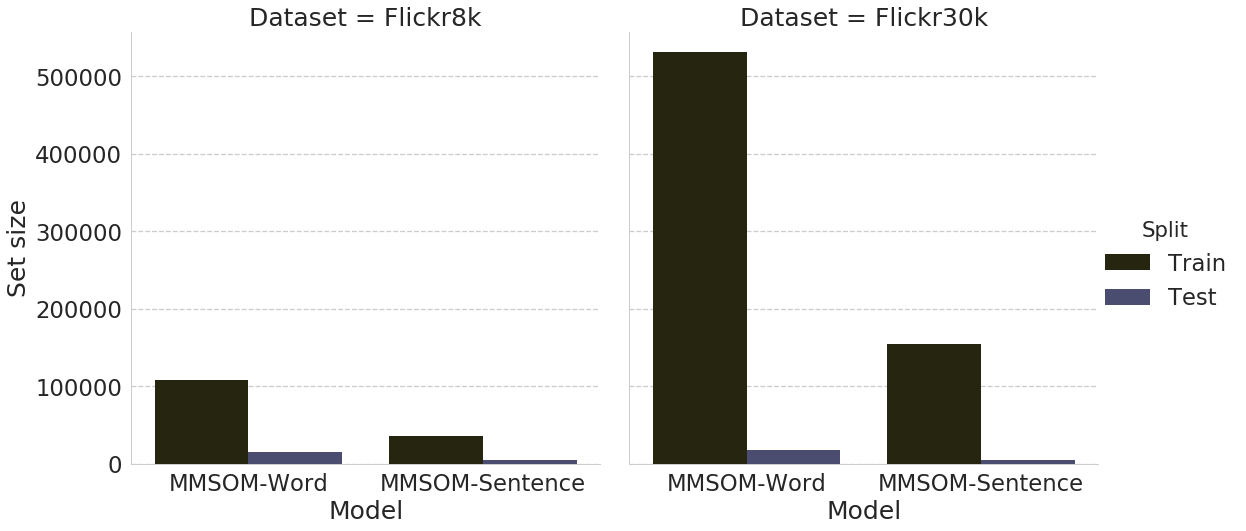
\includegraphics[width=\textwidth]{images/image_retrieval_data_info.png}
    \caption{Train and test sizes of the datasets used for the image retrieval experiments.}
    \label{fig:ImageRetrievalDatasetSizes}
\end{figure}

\begin{table}[h]
    \centering
    \begin{footnotesize}
        \begin{tabularx}{\textwidth}{|X|c|c|c|}
            \hline
            Model                           & Dataset  & Train set size & Test set size \\
            \hline
            \multirow{2}{*}{MMSOM-Word}     & Flikr8K  & 108,490        & 15,172         \\ 
            \cline{2-4}                     & Flikr30K & 530,682        & 17,391         \\ 
            \hline
            \multirow{2}{*}{MMSOM-Sentence} & Flikr8K  & \ \:35,416     & \ \:5000        \\
            \cline{2-4}                     & Flikr30K & 153,915        & \ \:5000        \\
            \hline
        \end{tabularx}
    \end{footnotesize}
    \caption{Train and test sizes of the datasets used for the image retrieval experiments.}
    \label{tab:ImageRetrievalDatasetSizes}
\end{table}

\begin{figure}[h]
    \centering
    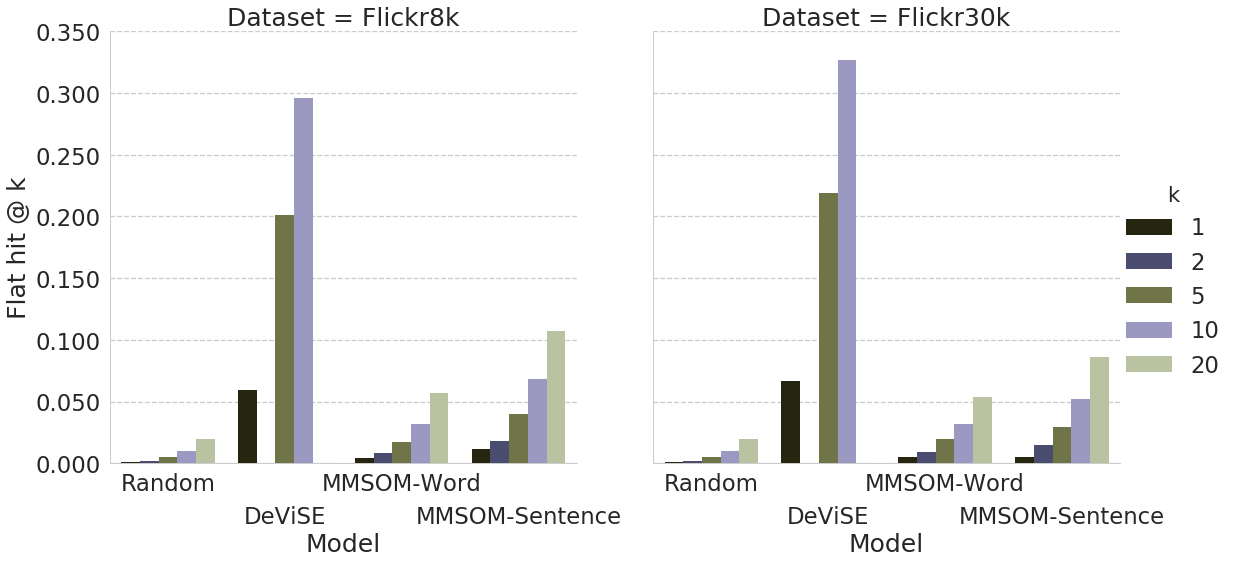
\includegraphics[width=\textwidth]{images/image_retrieval_results.png}
    \caption{Results for the image retrieval experiments. The results for the \texttt{DeViSE} model were reported in \cite{karpathy2014deep}.}
    \label{fig:ImageRetrievalResults}
\end{figure}

\begin{table}[h]
    \begin{footnotesize}
        \begin{tabularx}{\textwidth}{|X|c|c|c|c|c|c|}
            \hline
            \multirow{2}{*}{Model}          & \multirow{2}{*}{Dataset} & \multicolumn{5}{c|}{Flat hit @ $k$} \\
            \cline{3-7}                     &                          & 1      & 2      & 5      & 10     & 20     \\ 
            \hline
            \multirow{2}{*}{Random}         & Flickr8K                  & 0.0010 & 0.0020 & 0.0050 & 0.0100 & 0.0200 \\ 
            \cline{2-7}                     & Flickr30K                 & 0.0010 & 0.0020 & 0.0050 & 0.0100 & 0.0200 \\ 
            \hline
            \multirow{2}{*}{DeViSE}\cite{frome2013devise}
                                            & Flickr8K                  & \textbf{0.0590} & ------ & \textbf{0.2010} & \textbf{0.2960} & ------ \\ 
            \cline{2-7}                     & Flickr30K                 & \textbf{0.0670} & ------ & \textbf{0.2190} & \textbf{0.3270} & ------ \\ 
            \hline
            \multirow{2}{*}{MMSOM-Word}     & Flickr8K                  & 0.0040 & 0.0085 & 0.0173 & 0.0316 & 0.0566 \\ 
            \cline{2-7}                     & Flickr30K                 & 0.0055 & 0.0091 & 0.0194 & 0.0321 & 0.0536 \\ 
            \hline
            \multirow{2}{*}{MMSOM-Sentence} & Flickr8K                  & 0.0114 & 0.0180 & 0.0396 & 0.0680 & 0.1072 \\ 
            \cline{2-7}                     & Flickr30K                 & 0.0054 & 0.0146 & 0.0296 & 0.0518 & 0.0864 \\ 
            \hline
        \end{tabularx}
    \end{footnotesize}
    \caption{Results for the image retrieval experiments. The results for the \texttt{DeViSE} model were reported in \cite{karpathy2014deep}.}
    \label{tab:ImageRetrievalResults}
\end{table}

\subsection{Analysis and interpretation of results}\label{subsec:ImageRetrievalAnalysis}

The results clearly show that our approach was not appropriate for this task. One possible reason could lie in our training procedure. \Figref{Flickr30kWordFreq} shows the distribution of word frequencies for the Flickr30K dataset. As we can see, most of the words have a very low frequency, with a few having a relatively high frequency. Given the training procedure of the SOM, this could lead to the SOM-units corresponding to high frequency words converging correctly, while the SOM-units corresponding to low frequency words cannot converge.

\begin{figure}[h]
    \centering
    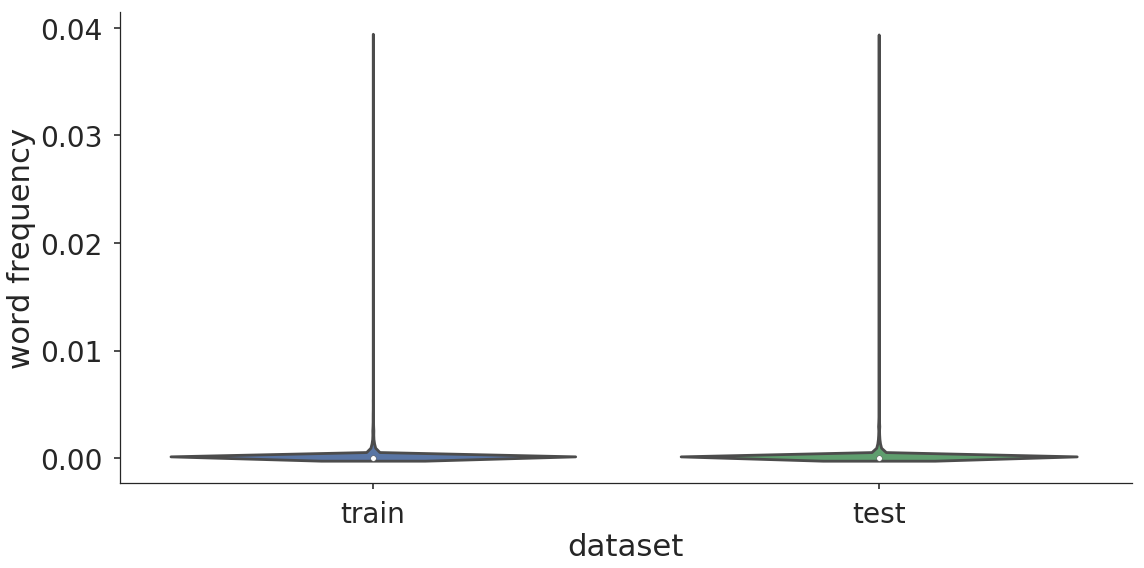
\includegraphics[width=\textwidth]{images/flickr30k_word_frequency.png}
    \caption{Word frequency distributions in the training and test datasets for Flickr30K, using the \texttt{MMSOM-Word} model. A higher word frequency means that the word was present in more sentences.}
    \label{fig:Flickr30kWordFreq}
\end{figure}

Possible solutions include augmenting the dataset to correct the imbalance, modifying the learning rate of the SOM training procedure according to the inverse of the word frequency, or using a completely different vector quantization method.

One more thing to take into account is the suitability of our performance measure. \Figref{ImageRetrievalStreetFail} shows some of the images retrieved for the query word "street" by the \verb|SOM-Sentence| model from the Flickr30K test set, with their descriptions at the top. As we can see, none of the descriptions contain the query word. Nonetheless, every scene takes place in a street setting. These cases would count as retrieval failures for the "flat hit @ $k$" measure, even though they seem to be correct. An alternative performance metric could be the "hierarchical hit @ k", explained in \secref{ZeroShotLearning}, \eqref{h_at_k}. The results for low values of $k$ are improved by using this metric, as shown in \tabref{ImageRetrievalHierarchical} for the \verb|MMSOM-Word| model on the Flickr8K dataset. A notion of why "hierarchical hit @ k" could be useful for image retrieval can be seen in \figref{ImageRetrievalSynsets}. The textual description of a retrieved image could contain any of the nodes in the graph, without containing the literal "street", and still be considered a relevant result for the query "street" by a human.
However, we have not found references of it being used in literature in this way, therefore its applicability in image retrieval is open to question.

\begin{figure}[h]
    \centering
    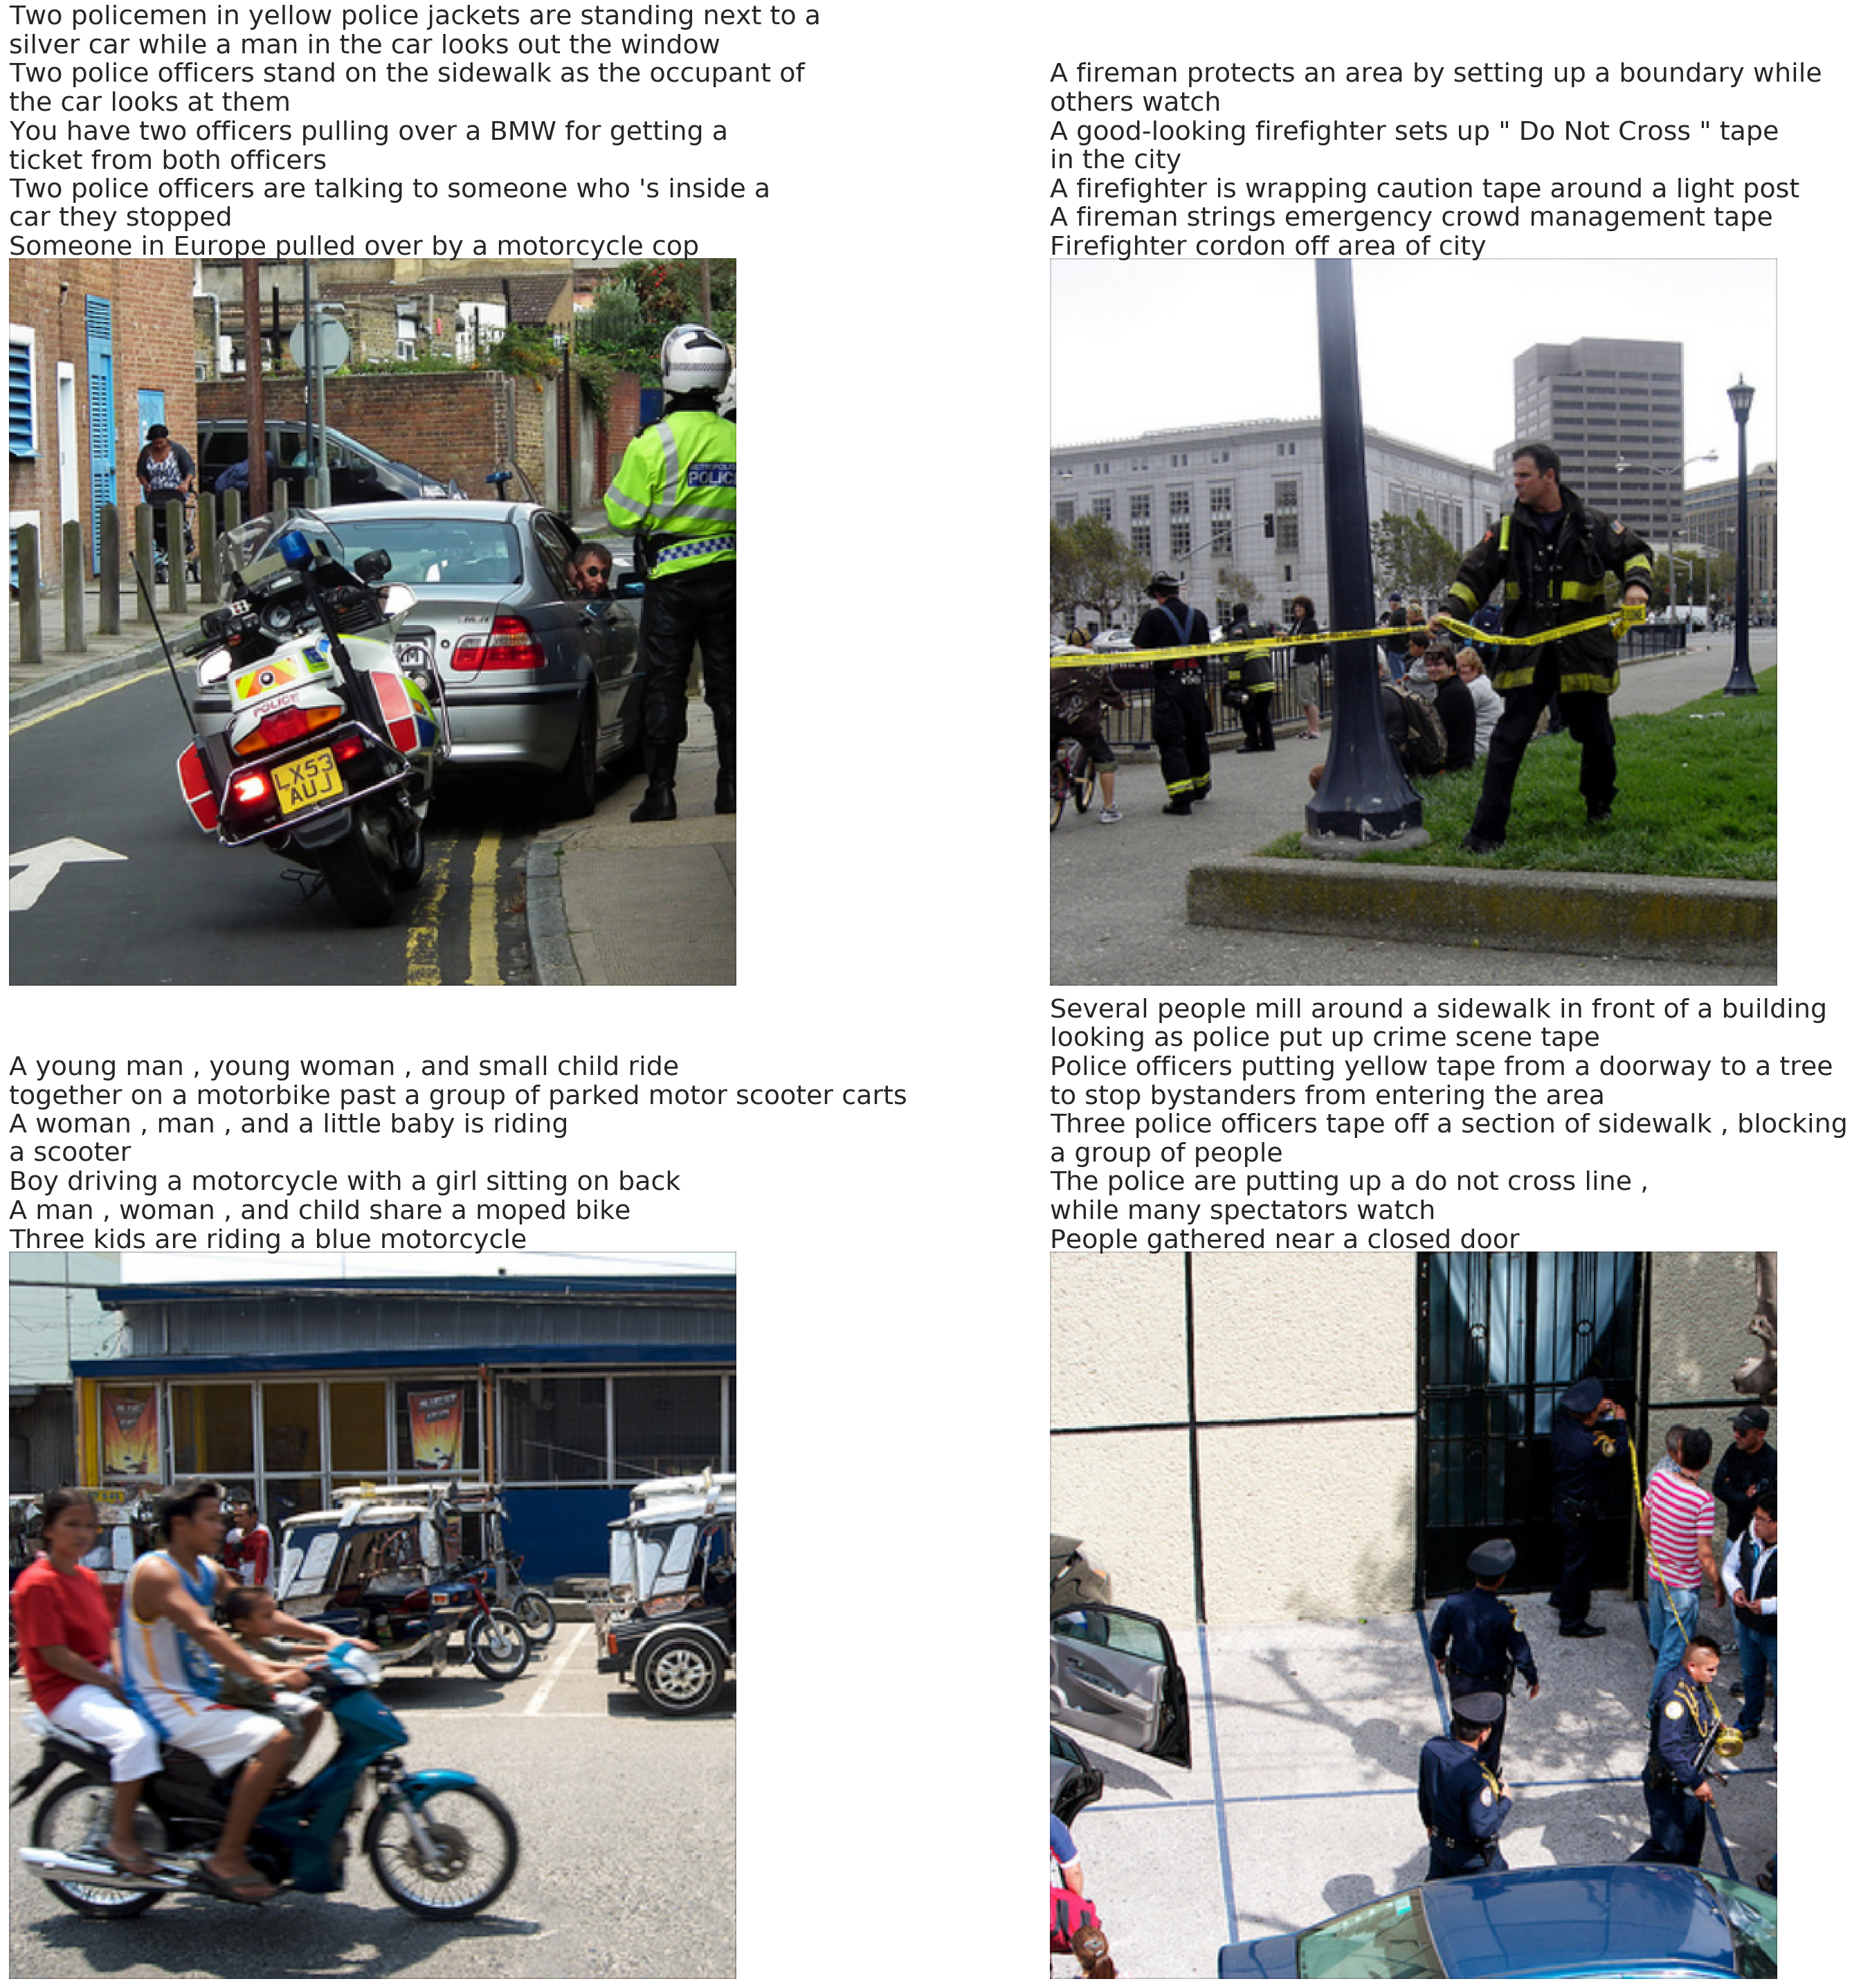
\includegraphics[width=\textwidth]{images/image_retrieval_street_fail.png}
    \caption{Images retrieved for the query word "street" by the \texttt{SOM-Sentence} model from the Flick30K test set}
    \label{fig:ImageRetrievalStreetFail}
\end{figure}

\begin{figure}[h]
    \centering
    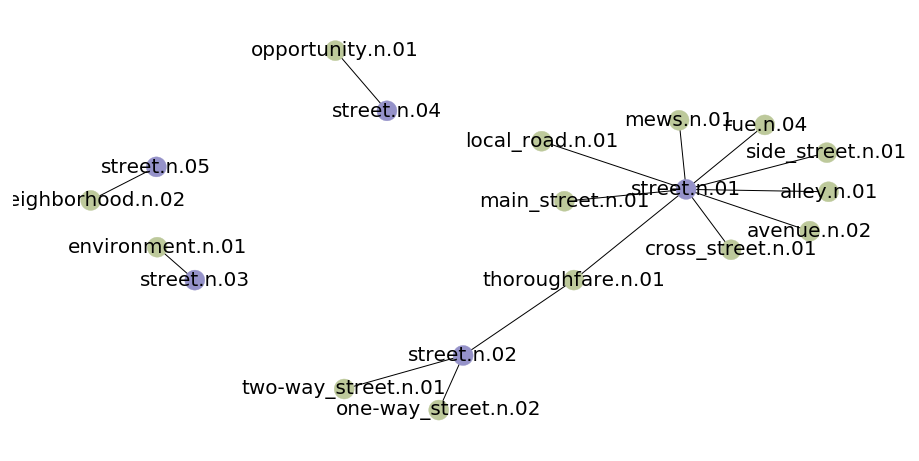
\includegraphics[width=\textwidth]{images/image_retrieval_fail_synsets.png}
    \caption{Hypernym-Hyponym closure (in orange) for the WordNet synsets corresponding to the word "street" (in green).}
    \label{fig:ImageRetrievalSynsets}
\end{figure}

\begin{table}[h]
    \begin{footnotesize}
        \begin{tabularx}{\textwidth}{|X|c|c|c|c|c|}
            \hline
            \multirow{2}{*}{Performance metric} & \multicolumn{5}{c|}{Flat hit @ $k$} \\
            \cline{2-5}                         & 1      & 2      & 5      & 10     & 20       \\ 
            \hline
            Flat hit @ k                        & 0.0040 & 0.0085 & 0.0173 & 0.0316 & 0.0566   \\ 
            \hline
            Hierarchical hit @ k                & N/A    & 0.0270 & 0.0282 & 0.0264 & 0.0189   \\ 
            \hline
        \end{tabularx}
    \end{footnotesize}
    \caption{Comparison of results using the "Flat hit @ k" vs "Hierarchical hit @ k" performance metrics for the \texttt{MMSOM-Word} model on the Flickr8K dataset.}
    \label{tab:ImageRetrievalHierarchical}
\end{table}

Given the sizes of the image embeddings relative to the word embeddings (4096 vs. 300) and our choice of distance metric, the images are going to have a \textasciitilde 13 times the weight of the words in any distance calculation. This effect could be offset by dividing each embedding by its length\footnote{$new\_img\_emb = img\_emb/4096; new\_wrd\_emb = wrd\_emb/300; $}, or by normalizing each embedding to unit euclidean norm before concatenation\footnote{$new\_img\_emb = img\_emb/\Vert img\_emb \Vert_2; new\_wrd\_emb = wrd\_emb/\Vert wrd\_emb \Vert_2; $}. We explored these alternatives using the \verb|MMSOM-Word| model on the Flickr8K dataset, but found that they provided worse results. We also tried to use the neighborhood relationships in the SOM by retrieving, for each of the k best matching units (BMUs) in the SOM, the single image in the test dataset nearest to that BMU\footnote{In of our final procedure we retrieved the k nearest images in the test dataset nearest to the the single BMU in the SOM}. This approach also provided worse results than our final procedure. The results of these failed alternatives are shown in \figref{ImageRetrievalFailed} and \tabref{ImageRetrievalFailed}. In light of this, we decided to avoid re-scaling the embeddings, normalizing them to unit lenght or using the SOM neighborhood in our final experiments.

\begin{figure}[h]
    \centering
    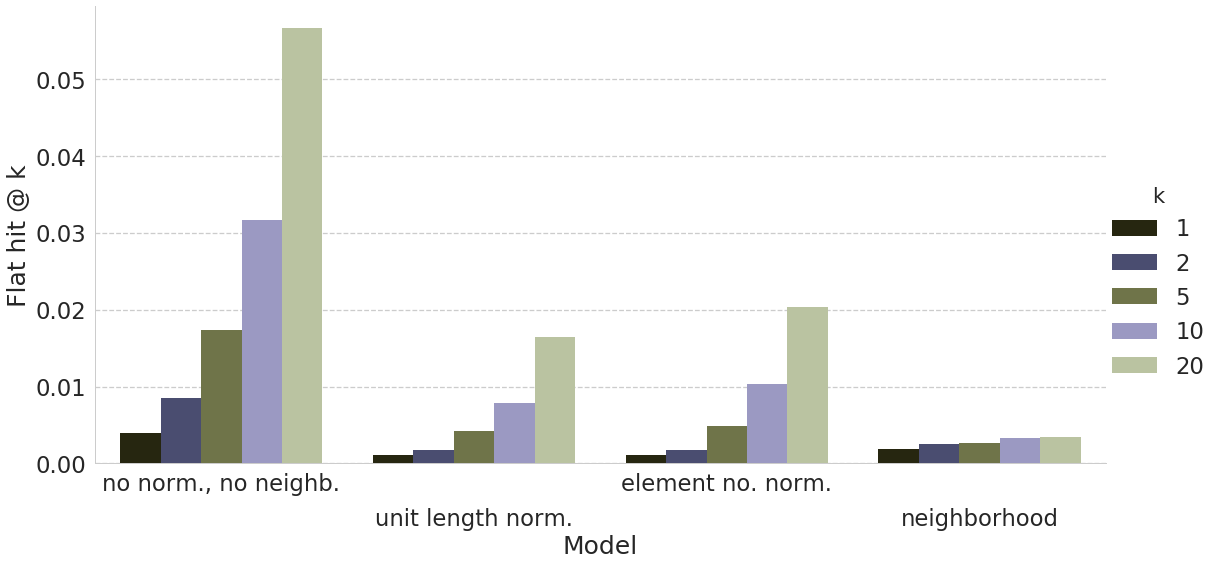
\includegraphics[width=\textwidth]{images/image_retrieval_fail_results.png}
    \caption{Results for the some failed approaches to the image retrieval experiments. \texttt{no norm, no neighb.}, \texttt{unit length norm.}, \texttt{element no. norm.} and \texttt{neighborhood} correspond, respectively, to \texttt{MMSOM-Word (no normalization, no neighborhood)}, \texttt{MMSOM-Word (unit length normalization)}, \texttt{MMSOM-Word (division by number of elements)} and \texttt{MMSOM-Word (neighborhood)} in \tabref{ImageRetrievalFailed}.}
    \label{fig:ImageRetrievalFailed}
\end{figure}

\begin{table}[h]
    \begin{footnotesize}
        \begin{tabularx}{\textwidth}{|X|c|c|c|c|c|}
            \hline
            \multirow{2}{*}{Model}                         & \multicolumn{5}{c|}{Flat hit @ $k$}        \\
            \cline{2-6}                                    & 1      & 2      & 5      & 10     & 20     \\ 
            \hline
            MMSOM-Word (no normalization, no neighborhood) & 0.0040 & 0.0085 & 0.0173 & 0.0316 & 0.0566 \\ 
            \hline
            MMSOM-Word (unit length normalization)         & 0.0011 & 0.0017 & 0.0042 & 0.0079 & 0.0165 \\ 
            \hline
            MMSOM-Word (division by number of elements)    & 0.0011 & 0.0018 & 0.0049 & 0.0103 & 0.0203 \\ 
            \hline
            MMSOM-Word (neighborhood)                      & 0.0019 & 0.0025 & 0.0027 & 0.0033 & 0.0034 \\ 
            \hline
        \end{tabularx}
    \end{footnotesize}
    \caption{Results for the some failed approaches to the image retrieval experiments. \texttt{MMSOM-Word (no normalization, no neighborhood)} is our final approach, shown in \tabref{ImageRetrievalResults}. \texttt{MMSOM-Word (unit length normalization)} normalizes the embedding of each modality to unit length individually. \texttt{MMSOM-Word (division by number of elements)} divides the image embedding by 4096 and the word embedding by 300. \texttt{MMSOM-Word (neighborhood)} retrieves, for each of the k BMUs in the SOM, the single image in the test dataset nearest to that BMU.}
    \label{tab:ImageRetrievalFailed}
\end{table}

\end{document}